\documentclass[14pt,aspectratio=169]{beamer}

\usepackage[utf8]{inputenc}
\usepackage{amsmath, amssymb, amsfonts, cancel}
\usefonttheme[onlymath]{serif}
\usetheme{Warsaw}
\setbeamertemplate{navigation symbols}{}
\setbeamertemplate{headline}{}
\setbeamercovered{transparent}
\mode<presentation>

\begin{document}

\title{Session 2 : The Conic Sections}
\subtitle{\textit{Precalculus: A Problem-Solving Approach}}
\author{JING ARQUERO}
\institute{{\normalsize University of the East - Manila} \\ {\normalsize C.M. Recto Ave., Manila, Philippines}}
\date{All Rights Reserved {\textrm{\copyright}} 2019}

\begin{frame}
 \maketitle
\end{frame}

\begin{frame}{Session Outline}
    \begin{enumerate}
     \item History of Analytic Geometry
     \item The Cone
     \item The Double-Napped Cone
     \item The Conic Sections
     \item References
    \end{enumerate}

\end{frame}

\begin{frame}{A Brief History of Analytic Geometry}
    \begin{columns}
     \column{0.5\textwidth}
    \centering
     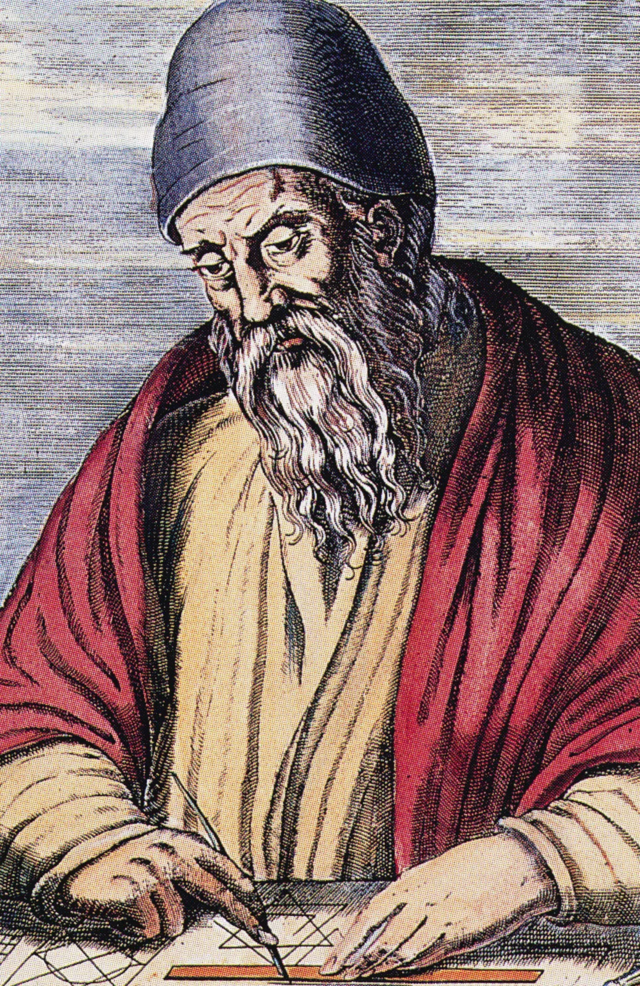
\includegraphics[width=0.5\textwidth]{image01.png}\\
     Euclid

     \column{0.5\textwidth}
        \begin{block}{Pre-Cartesian Era}
            \vspace{1mm}
            \begin{itemize}
             \item Geometry, 2000 B.C.
             \item No Cartesian Plane
             \item Plane Geometry \\
                    \textit{Two-Dimensional} (2D) \\
                    Point, Line, Plane
            \item Solid Geometry \\
                \textit{Three-Dimensional} (3D) \\
                    Cube, Sphere \textit{etc.}
            \end{itemize}
            \vspace{1mm}

        \end{block}

    \end{columns}

\end{frame}

\begin{frame}{A Brief History of Analytic Geometry}
 \begin{columns}

  \column{0.5\textwidth}
    \centering
        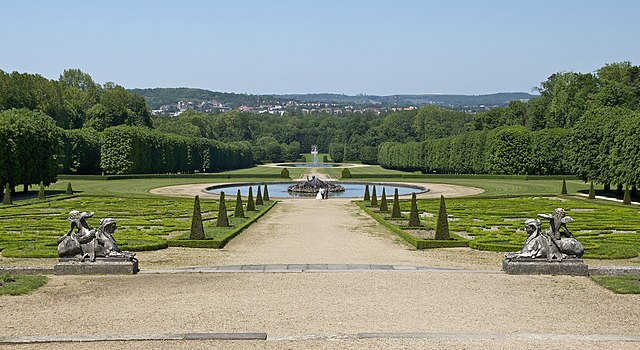
\includegraphics[width=1\textwidth]{image02.jpg} \\
        A fountain gets smaller as you move far away from it
  \column{0.5\textwidth}
    \begin{block}{Perspective Geometry}
        \vspace{1mm}
        \begin{itemize}
         \item 3D objects can be created from 2D Objects
         \item 2D objects can be derived from 3D Objects
         \item 3D objects and 2D objects can be manipulated${}^\text{1}$


        \end{itemize}
        \vspace{1mm}

    \end{block}
    {\footnotesize ${}^\text{1}$\textit{Translated, Rotated, Dilated, Contracted, Sliced, Destroyed, Recreated, Transformed}}

 \end{columns}

\end{frame}

\begin{frame}{A Brief History of Analytic Geometry}
    \begin{columns}
    \column{0.5\textwidth}
    \centering
    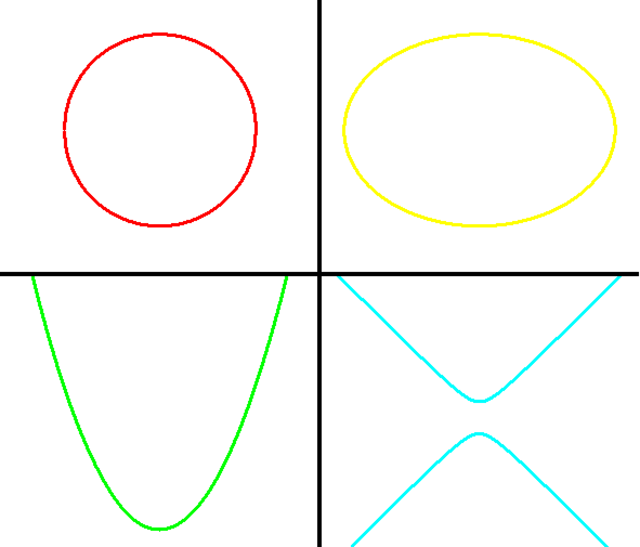
\includegraphics[width=0.9\textwidth]{image03.png}\\
    The Two-Dimensional Curves
    \column{0.5\textwidth}
    \begin{block}{Existence of 2D Curves}

        \begin{itemize}
         \item Ellipse
         \item Circle
         \item Parabola
         \item Hyperbola
        \end{itemize}

    \end{block}

    \begin{exampleblock}{Geometric Realization}
        \textit{Since 2D objects are derived from 3D objects, what 3D object contains all the curves?}
    \end{exampleblock}

    \end{columns}


\end{frame}

\begin{frame}{A Brief History of Analytic Geometry}
    \begin{columns}
     \column{0.5\textwidth}
     \centering
     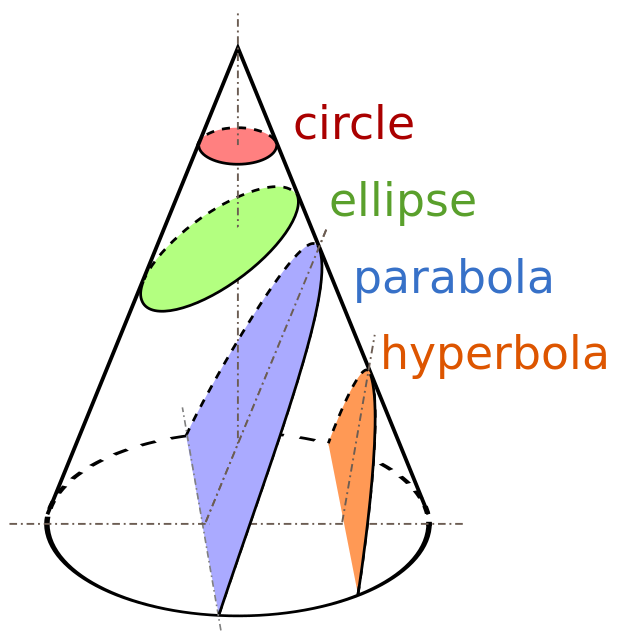
\includegraphics[width=0.8\textwidth]{image04.png} \\
     The Cone and the Conic Sections
     \column{0.5\textwidth}
     \begin{block}{The Cone \& The Conic Sections}
        \vspace{1mm}
        \begin{itemize}
         \item Menaechmus (\textit{c. 355 B.C.})
         \item A \textbf{Cone} is a 3D object that tapers from a circular base to a point
         \item The curves are derived by slicing a cone
         \item The curves, being derived parts from a cone, is now called \textbf{Conic Sections}
        \end{itemize}
        \vspace{1mm}


     \end{block}

    \end{columns}

\end{frame}


\begin{frame}{The Cone \& The Conic Sections}
 \begin{columns}
  \column{0.5\textwidth}
    \centering
     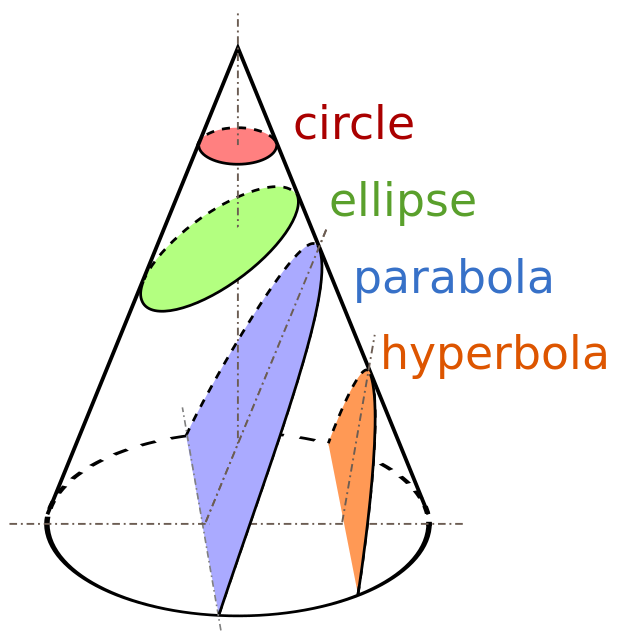
\includegraphics[width=0.8\textwidth]{image04.png} \\
     The Cone and the Conic Sections
  \column{0.5\textwidth}
    \centering
    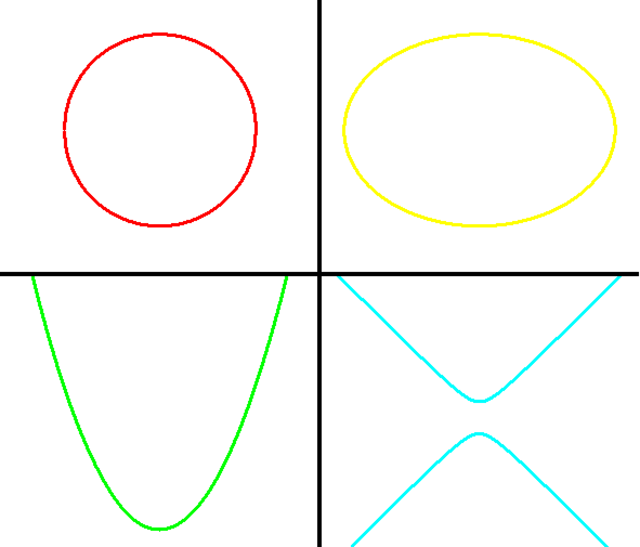
\includegraphics[width=0.9\textwidth]{image03.png}\\
    The Two-Dimensional Curves

 \end{columns}

\end{frame}

\begin{frame}{The Iconic Mistake}
    \begin{columns}
     \column{0.5\textwidth}
        \centering
        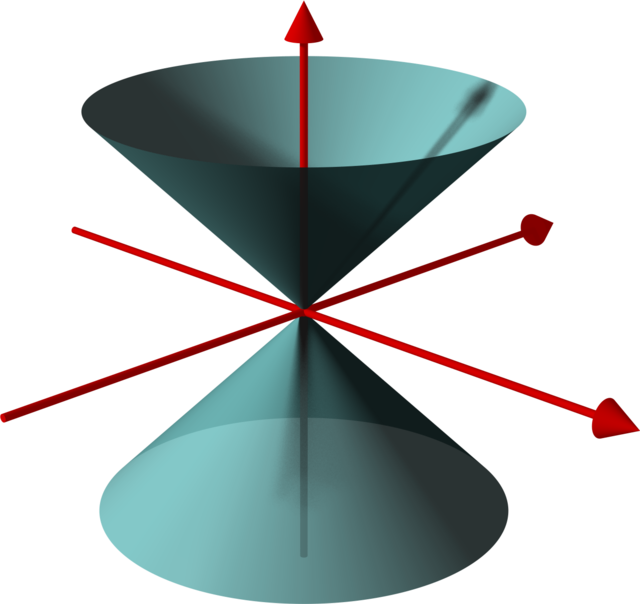
\includegraphics[width=0.8\textwidth]{image05.png}\\
        The Double-Napped Cone
     \column{0.5\textwidth}
        \begin{block}{The Double-Napped Cone}
        \vspace{1mm}
         \begin{itemize}

          \item The Hyperbola has two distinct branches
          \item A cone has one branch
          \item In resolution, another cone was put atop of the other
          \item Apollonius (\textit{c. 240 B.C.})
          \item Analytic Geometry was born
          \item The Conic Equations
         \end{itemize}
         \vspace{1mm}

        \end{block}

    \end{columns}


\end{frame}



\begin{frame}{The Double-Napped Cone}
    \centering
    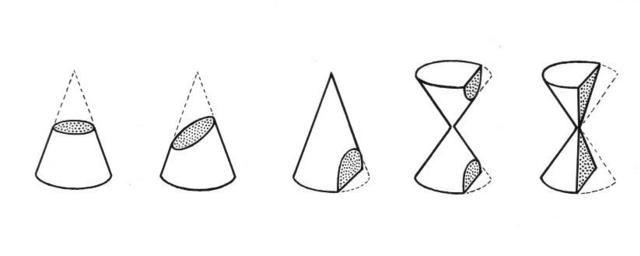
\includegraphics{image06}\\
    Conic Sections on the Double-Napped Cone


\end{frame}

\begin{frame}{People in History}
 \begin{columns}
  \column{0.5\textwidth}
  \centering
    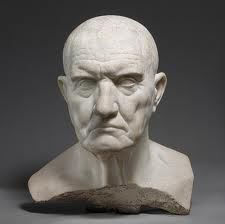
\includegraphics[width=0.9\textwidth]{image07.jpeg}\\ Menaechmus

  \column{0.5\textwidth}
  \centering
    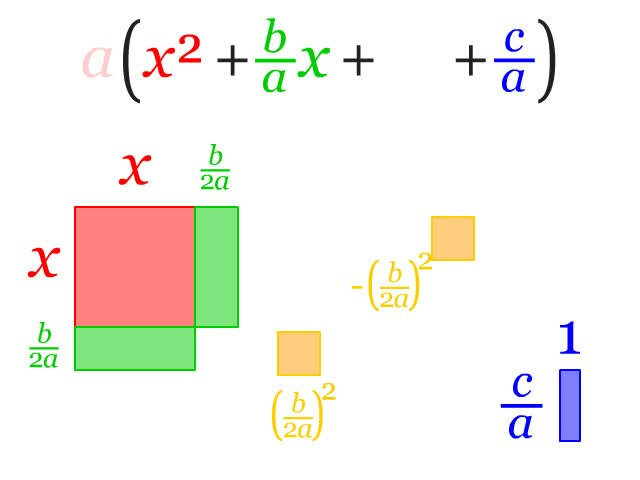
\includegraphics[width=0.9\textwidth]{image08.jpg}\\ Apollonius of Perga

 \end{columns}

\end{frame}



\begin{frame}{Circle \& Ellipse}
 \begin{columns}
     \column{0.5\textwidth}
     \begin{block}{Definition}
      A circle is obtained by slicing a double-napped cone with a plane parallel to the base of the cone.
     \end{block}
\begin{block}{Definition}
      An ellipse is obtained by slicing a double-napped cone with a tilted plane intersecting only one of the cones.

     \end{block}
     \column{0.5\textwidth} \centering
        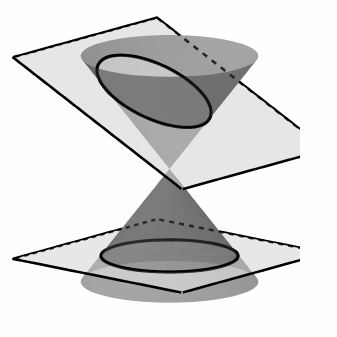
\includegraphics[width=0.8\textwidth]{image08.png}\\Circle and Ellipse
    \end{columns}
\end{frame}


\begin{frame}{Parabola}
 \begin{columns}
     \column{0.5\textwidth}
          \begin{block}{Definition}
      A parabola is obtained by slicing a double-napped cone with a plane parallel to the edges of the cones.
     \end{block}
     \column{0.5\textwidth} \centering
        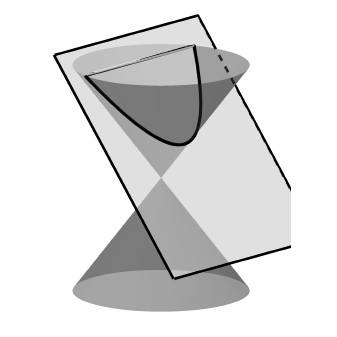
\includegraphics[width=0.8\textwidth]{image09.png}\\Parabola

    \end{columns}

\end{frame}



\begin{frame}{Hyperbola}
 \begin{columns}
     \column{0.5\textwidth}
    \begin{block}{Definition}
     \vspace{1mm}
      A hyperbola is obtained by slicing a double-napped cone with a plane intersecting both cones.
      \vspace{1mm}
     \end{block}
     \column{0.5\textwidth}\centering
        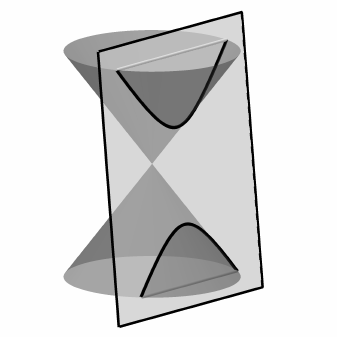
\includegraphics[width=0.8\textwidth]{image10.png}\\Hyperbola

    \end{columns}

\end{frame}

\begin{frame}{Degenerate Conic Sections}
 \centering
        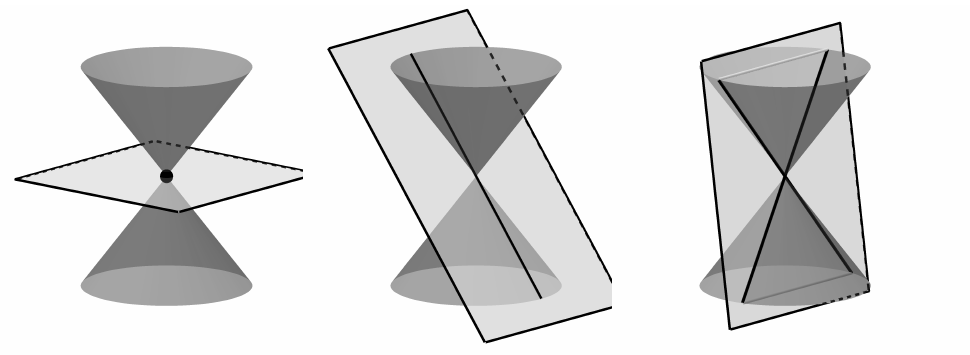
\includegraphics[width=0.8\textwidth]{image11.png}\\Point, Line, Intersecting Lines
\end{frame}

\begin{frame}{The Conic Equations}
 \begin{columns}
  \column{0.5\textwidth}\centering
  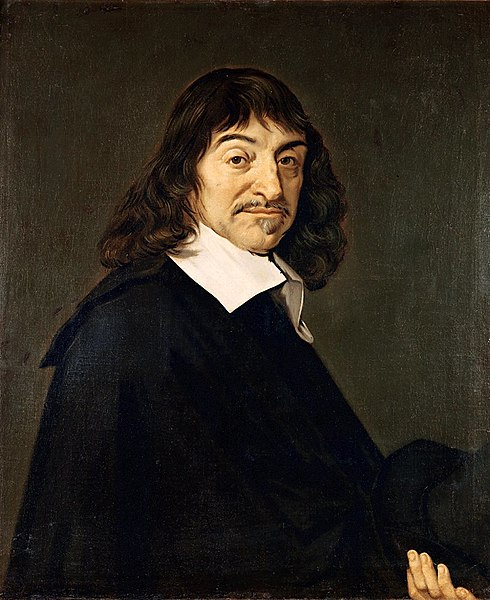
\includegraphics[width=0.5\textwidth]{image12.jpg}\\Rene Descartes
  \column{0.5\textwidth}
  \begin{block}{The Cartesian Era}
   \begin{itemize}
    \item The Rectangular Coordinate System
    \item Simplified perspectives of 3D Objects
    \item Later, The Cartesian Plane
   \end{itemize}

  \end{block}

  \begin{block}{The Conic Equation}
   $Ax^2 + By^2 + Cx + Dy + E = 0$
  \end{block}

 \end{columns}

\end{frame}

\begin{frame}{General Equation of a Circle}
 \begin{columns}
     \column{0.5\textwidth} \centering
        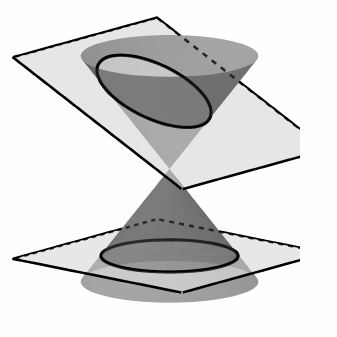
\includegraphics[width=0.8\textwidth]{image08.png}\\Circle and Ellipse
     \column{0.5\textwidth}
        \begin{block}{Equation of a Circle}\centering
        $A=B$, A,B $>0$  \\
        \end{block}

        \begin{exampleblock}{Examples}
         $4x^2 + 4y^2 + 8x + 20y + 1 = 0$ \\
         $3x^2 +3y^2 + 12x - 6y - 11 = 0$
        \end{exampleblock}

    \end{columns}
\end{frame}

\begin{frame}{General Equation of an Ellipse}
 \begin{columns}
     \column{0.5\textwidth} \centering
        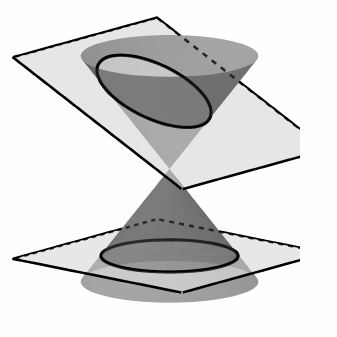
\includegraphics[width=0.8\textwidth]{image08.png}\\Circle and Ellipse
     \column{0.5\textwidth}
        \begin{block}{Equation of an Ellipse}\centering
        $A\neq B$; liked signed, not $0$
        \end{block}

        \begin{exampleblock}{Examples}
         $4x^2 + 5y^2 + 8x + 20y + 1 = 0$ \\
         $-x^2 - 2y^2 + 12x - 6y - 11 = 0$
        \end{exampleblock}

    \end{columns}
\end{frame}

\begin{frame}{General Equation of a Parabola}
 \begin{columns}
     \column{0.5\textwidth} \centering
        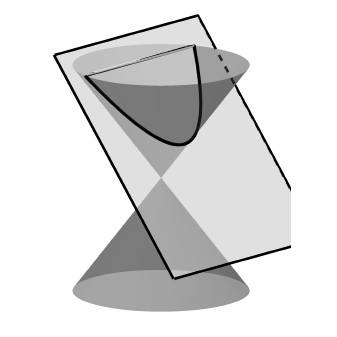
\includegraphics[width=0.8\textwidth]{image09.png}\\Parabola
     \column{0.5\textwidth}
        \begin{block}{Equation of a Parabola} \centering
        $A,B=0$, but not both  \\
        \end{block}

        \begin{exampleblock}{Examples}
         $4x^2 + 8x + 20y + 1 = 0$ \\
         $-2y^2 + 12x - 6y - 11 = 0$
        \end{exampleblock}

    \end{columns}
\end{frame}

\begin{frame}{General Equation of a Hyperbola}
 \begin{columns}
     \column{0.5\textwidth} \centering
        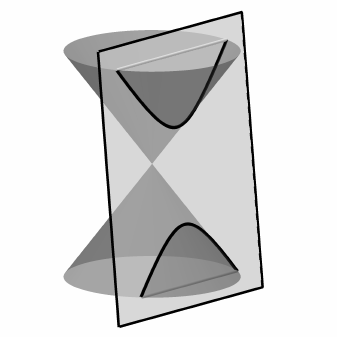
\includegraphics[width=0.8\textwidth]{image10.png}\\Hyperbola
     \column{0.5\textwidth}
        \begin{block}{Equation of a Parabola}\centering
        $A,B=0$, but opposite signs  \\
        \end{block}

        \begin{exampleblock}{Examples}
         $4x^2 - 8y^2 + 8x + 20y + 1 = 0$ \\
         $-x^2 + 2y^2 + 12x - 6y - 11 = 0$
        \end{exampleblock}

    \end{columns}
\end{frame}

\begin{frame}{General Equations of Degenerate Sections}
\begin{columns}
 \column{0.5\textwidth}
 \centering
        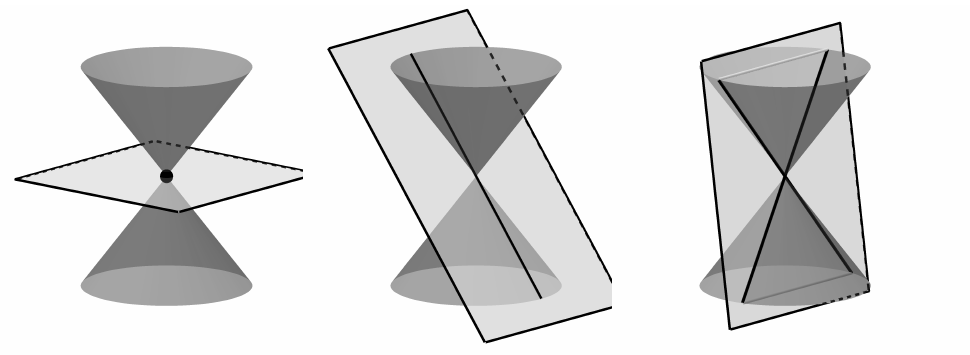
\includegraphics[width=0.8\textwidth]{image11.png}\\Point, Line, \\ Double-Napped Triangle
 \column{0.5\textwidth}
 \begin{exampleblock}{Examples}
  \textbf{Point} \\
  $2x^2 + 5y^2 + 12x -20y + 38 =0$ \\~\\
  \textbf{Double-Napped Triangle}\\
  $2x^2-3y^2-20x-18y+23=0$\\~\\
  \textbf{Complex Graph} \\
  $x^2+y^2+2x-6y+15=0$
 \end{exampleblock}

\end{columns}

\end{frame}

\begin{frame}{Seatwork}
\textbf{GENERAL DIRECTIONS:}
\begin{itemize}
 \item Only write with a black-inked ballpoint pen
 \item Read the instructions and problems carefully
 \item Legibly write your solutions, and box your final answers
 \item Avoid cheating, using devices, and making erasures
 \item Physical Scientific Calculators are allowed
\end{itemize}

 \begin{block}{IT'S YOUR TURN}
    Answer \emph{pg. 11} Nos. 1 - 3
 \end{block}

 \begin{block}{HOW CLEAR IS THE LESSON TO YOU?}
  Answer \emph{pg. 12} Nos. 9 - 12 \& Nos. 14 - 20
 \end{block}


\end{frame}




\begin{frame}{References}
\textbf{DOCUMENTATION}\\
 This slide presentation is made with {\textrm \LaTeX}.
 The source code is available at:
 \texttt{https://github.com/redundies/ueshsprecal}\\~\\

 \textbf{REFERENCES}
 \begin{itemize}
  \item Garces, Ian June et. al (2016) \textit{Precalculus: Specialized Subject}
  \item Tamayo, Joycelyn et. al (2018) \textit{Precalculus for SHS Students}
  \item De Guzman, Danilo et. al (2019) \textit{Precalculus: A Worktext}
  \item Most Images from (\texttt{https://wikimedia.com}), {\sc PD-CC0L}
 \end{itemize}


\end{frame}


\end{document}
